\begin{figure}[h!]
\centering
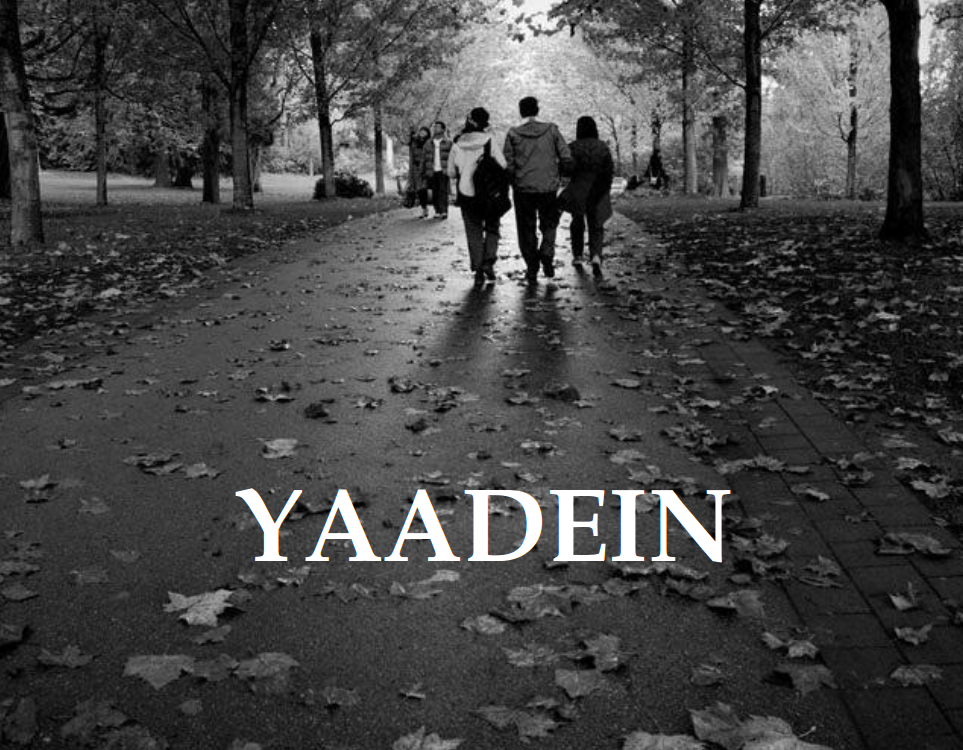
\includegraphics[width=0.9\textwidth]{images/souvenir.png}
\caption{Yaadein}
\end{figure}
\hspace{-1.8em} Yaadein or souvenir or memories is a great application to produce web based as well as printed copies
of souvenirs which are given to students when they pass out from schools and colleges.
It con- tains every students personal details, photograph, contact details and the com-
ments/views of other students about them.\\\\
A SOUVENIR from French, for a remembrance or memory, memento, keepsake or
token of remembrance is an object a person acquires for the memories the owner asso-
ciates with it.\\\\
Yaadein was made keeping in mind the various schools and colleges who spend several
man hours, which often run into days and sometimes weeks, designing their souvenir.
This project will not only help them significantly reduce the time consumed in the de-
signing of the souvenir but will also make the overall process very simple and easy to
use. The Yaadein project is a highly customizable application that allows the user to
modify the look and feel of the souvenir as per their personal preferences.\\\\
Software developed not only automate the Typesetting of the Souvenir but also does
the imposition and colour separation which are done by the printer before printing the
souvenir.\\\\
Imposition is one of the fundamental steps in the prepress printing process. It con-
sists in the arrangement of the printed products pages on the printers sheet, in order to
obtain faster printing, simplified binding and less waste of paper.\\\\
Correct imposition minimizes printing time by maximizing the number of pages per
impression, reducing cost of press time and materials. To achieve this, the printed sheet
must be filled as fully as possible.\\\\
Imposition is affected by five different parameters:\\
\begin{itemize}
\item Format of the product: The size of the finished page determines how many pages
can be printed on a single sheet.
\item Number of pages of the printed product: The compositor must determine how
many sheets are to be printed to create a finished book.
\item Stitching/binding method: The compositor must understand how the sheets are
placed to form the signatures that compose the finished book.
\item Paper fiber direction: Many papers have a ”grain,” reflecting the alignment of the
paper fibers. That these fibers must run lengthwise along the fold influences the
alignment, hence the position, of the pages on the printed sheet.
\item Finishing and binding
\end{itemize}
To understand how the pages are related to each other, an imposition dummy may be
used. This is made by folding several sheets of paper in the way the press will print and
fold the product. A little copy is then created, and this can help paginate the product.\\\\
\image{0.9}{images/imposition.png}{Imposition of 16 pages}\\\\
\hspace{-1.8em} Also, this project is completely open source and is made using PhP, \LaTeX{} version
\LaTeX{}2e and MySql and the entire code is available to the user as and when required.
The project is governed by the GNU General Public License v3.0 i.e GNU-GPLv3.0.\\\\
Various tools used to develop the project are:\\
\begin{itemize}
\item phpMyadmin
\item PHP
\item MySQL
\item \LaTeX{}
\item GIMP
\item ImageMagick
\end{itemize}

\subsection{Software requirements}
\begin{itemize}
\item Operating System: Linux/Windows
\item Programming Language: PHP
\item Mysql
\item \LaTeX{} Typesetting Editor
\end{itemize}

\subsection{Hardware Requirements}
Hardware requirement of this project is any Desktop or Laptop machine for local
use or a Server with minimum available configuration to make Project globally
available. Hardware specifications of the machine used depends upon the hardware
requirements of the Operating System installed on it. As such there are no special
hardware requirements of this project.\\
